\part{El proceso}

\section{Conceptos}

\paragraph{Ingeniería del Software} Aplicación de un enfoque sistemático, disciplinado y cuantificable hacia el desarrollo, operación y mantenimiento del software; es decir, la aplicación de la ingeniería al software. (IEEE). Es necesaria para identificar y conocer las causas de los problemas en el desarrollo del software, combinando las metodologías necesarias, dado que no van a desaparecer de la noche a la mañana. Está implícita la existencia de fases, de modo que la ingeniería del software proporciona una metodología que indica en cada momento los pasos a seguir, así como permite identificar en qué parte del proceso de ingeniería estamos y cuán bien lo estamos haciendo.

%Adaptadas y añadadidas las definiciones del rabo de las traspas, de abajo a arriba porque es como tiene el rabo
\paragraph{Tarea} Cualquier acción que transforma una entrada en salidas, el objetivo debe de ser pequeño y bien definido. \textit{Ej: Ejecución del caso de prueba}.


\paragraph{Actividad} Conjunto de tareas que producen un producto importante del trabajo. \textit{Ejemplo: desarrollo de un plan de pruebas.}

\paragraph{Proceso} Conjunto de actividades, y tareas que se ejecutan para llevar a cabo algún producto de trabajo. Este conjunto es \textbf{adaptable} a las necesidades del que lo utiliza. \textit{Ejemplo: Validación}.


\paragraph{Modelo de los procesos} Descripción de los procesos involucrados en el desarrollo del software sin especificar cuando se desarrolla: \textit{Ejemplos: IEEE 1074, ISO 12207-1 e ISO/IEC TR 15504-2}.


\paragraph{Métodos y procedimientos} Determinan el modo en el que se \textit{ejecutan las tareas}, determinando qué técnicas se utilizan en cada fase y cómo. \textit{Ejemplo: IEEE 1008}.

\paragraph{Técnica} Cualquier recurso utilizado para llevar a cabo una tarea. Normalmente hablamos de gráficos con apoyos textuales.\textit{ Ej: Cobertura de caminos}.

\paragraph{Herramienta} Cualquier software que nos ayude en cualquier etapa del desarrollo. \textit{Ejemplo: JUnit}.

% TODO metodologia y ciclos de vida faltan o se han suprimido por algun motivo?


\section{Procesos para la construcción del software}


La construcción del software incluye una serie de actividades que se empiezan a estandarizar. \textit{Pressman} divide la construcción de software en \textbf{3 fases}:

\begin{enumerate}
    \item \textbf{Fase de definición}: Se centra en el \textbf{qué}, intentando identificar la información a procesar, la función y rendimiento esperados, las restricciones de diseño, las interfaces a utilizarse, los sistemas operativos y de hardware a utilizar, y los criterios de validación. Se identifican 3 actividades:
    \begin{itemize}
        \item \textbf{Análisis del sistema}: Define el papel de cada elemento relacionado con el sistema informático a desarrollar.
        \item \textbf{Análisis de requisitos del software}: Proporciona el ámbito del software y su relación con el resto de componentes del sistema.
        \item \textbf{Planificación}: Organización de las tareas que se llevarán a cabo en el proyecto.

        Es análisis y definición de requisitos es una tarea que debe ser llevada a cabo conjuntamente por el desarrollador de software y el cliente. \uline{Esta etapa produce el documento de especificación de requisitos del software.}
    \end{itemize}
    \item \textbf{Desarrollo}: Se intenta definir \textbf{cómo} han de diseñarse las estructuras de datos, cómo ha de implementarse la función dentro de una arquitectura software, cómo han de implementarse los detalles procedimentales, cómo han de caracterizarse las interfaces, cómo ha de traducirse el diseño en un lenguaje de programación y cómo han de realizarse la pruebas. Se definen 3 actividades: 
    \begin{itemize}
        \item \textbf{Diseño del software}.
        \item \textbf{Codificación}.
        \item \textbf{Pruebas}.
    \end{itemize}
    \item \textbf{Mantenimiento}: Se centra en el cambio asociado a la corrección de errores, a las adaptaciones requeridas a medida que evoluciona el entorno del software, y a los cambios debidos a las mejoras producidas por los requisitos cambiantes del cliente. Se definen 4 actividades:
    \begin{itemize}
        \item \textbf{Adaptación} (cambio del entorno).
        \item \textbf{Corrección} (errores).
        \item \textbf{Mejora} (cambios en los requisitos).
        \item \textbf{Prevención} (mejor ingeniería).
    \end{itemize}
\end{enumerate}

\textbf{Nota:} \textit{Estas actividades se aplican de forma iterativa según la última versión del Pressman. Por ejemplo un proceso de mantenimiento como puede ser la corrección de un error grande encajaría como una iteración de este modelo y no como una actividad concreta.}

\subsection{Norma IEEE 1074 -- 2006}
Proporciona el conjunto de actividades que constituyen los procesos que son necesarios para el correcto desarrollo y mantenimiento del software. Los procesos se dividen en 4 secciones lógicas:

\begin{enumerate}
    \item \textbf{Modelo del Ciclo de Vida Software}. Actividades para seleccionar el modelo de ciclo que \textbf{mejor se adapte} al proyecto; es necesario escoger uno. Además, la versión de 2006 requiere que se evalúe el riesgo.
    \item \textbf{Grupos de Actividades de Gestión del Proyecto}. Son los procesos que inician, supervisan y controlan los proyectos de software a lo largo de su ciclo de vida.
          \begin{itemize}
              \item \textbf{Iniciación del proyecto}: Se crea el ciclo de vida y se definen las métricas para la gestión del proyecto.
              \item \textbf{Planificación y control del proyecto}: Se desarrollan planes para la evaluación, gestión de la configuración, instalación, integración, etc.
              \item \textbf{Monitorización y control}: Actividades de gestión de riesgos, gestión de proyecto, mejoras del ciclo de vida, recolección y análisis de métricas, y cierre del proyecto.
          \end{itemize}
    \item \textbf{Grupos de Actividades Orientadas al desarrollo}. Comprenden los procesos que se realizan antes, durante y después del desarrollo software.
          \begin{itemize}
              \item Pre--desarrollo:
                    \begin{itemize}
                        \item Análisis de la necesidad del sistema.
                        \item Asignación de requisitos del sistema al software y al hardware (solo si se trabajará con ambos).
                    \end{itemize}
              \item Desarrollo:
                    \begin{itemize}
                        \item Análisis de requisitos.
                        \item Diseño de arquitectura, BBDD, interfaces\ldots
                        \item Implementación (codificación, documentación, integración, gestión de versiones\ldots).
                    \end{itemize}
              \item Post--desarrollo:
                    \begin{itemize}
                        \item Instalación.
                        \item Operación y Soporte.
                        \item Mantenimiento.
                        \item Retirada.
                    \end{itemize}
          \end{itemize}
    \item \textbf{Grupos de Actividades de Soporte}: Necesarios para asegurar terminación y \textbf{calidad de los procesos} y, por lo tanto, del proyecto.
          \begin{itemize}
              \item Verificación y Validación (aseguramiento de la calidad).
              \item Gestión de Configuración Software.
              \item Desarrollo de documentación.
              \item Formación.
          \end{itemize}
\end{enumerate}

\subsection{Norma ISO 12207--1}
Define una serie de actividades que se realizan en la construcción del software, agrupadas en \textbf{cinco procesos principales, ocho de soporte, y cuatro de la organización}. No fomenta ningún modelo concreto de ciclo de vida, gestión del software o método de ingeniería, ni prescribe cómo realizar las actividades o cómo organizarlas.

\subsubsection{Procesos principales}
Los procesos principales resultan útiles a las personas que inician o realizan el desarrollo, la explotación o el mantenimiento del software durante su ciclo de vida. Consisten en:
\begin{enumerate}
    \item \textbf{Proceso de adquisición}: Contiene las actividades realizadas por el cliente para adquirir un software. \textit{Ej: Solicitud de ofertas, o selección del suministrador}.
    \item \textbf{Proceso de suministro}: Contiene las actividades que realiza el suministrador. Incluye la preparación de la oferta para responder a una solicitud, y la identificación de los recursos y procedimientos para garantizar el éxito del proyecto.
    \item\textbf{Proceso de desarrollo}: Contiene numerosas actividades:
    \begin{itemize}
        \item \uline{Análisis de requisitos del sistema}: funcionales y no funcionales.
        \item \uline{Diseño de la arquitectura del sistema}: principales componentes de hardware y software.
        \item \uline{Análisis de los requisitos del software}: se definen y documentan (pruebas de aceptación).
        \item \uline{Diseño de la arquitectura del software}: se transforman los requisitos en una estructura de alto nivel en la que se pueden identificar los componentes principales. Se elabora una versión previa de los manuales, se define qué deben cumplir las pruebas de estos componentes, y se planifica la integración.
        \item \uline{Diseño detallado del software}: se diseña de forma detallada cada componente de software. Se actualizan los manuales, se define qué deben cumplir las pruebas de estos componentes, y se planifican las pruebas unitarias.
        \item \uline{Codificación y prueba}: se desarrollan y documentan los componentes software, y se prueba cada uno. Se actualizan los manuales.
        \item \uline{Integración del software}: se integran los componentes del software y se prueban según sea necesario. Se actualizan los manuales.
        \item \uline{Prueba del software}: en función de los requisitos especificados para él.
        \item \uline{Integración del sistema}: integración de elementos software y hardware.
        \item \uline{Prueba del sistema}: de acuerdo con los requisitos de cualificación especificados para el sistema.
        \item \uline{Instalación}: en el entorno de explotación final.
        \item \uline{Soporte del proceso de aceptación}: apoyo a la revisión de aceptación y prueba por parte del comprador.
    \end{itemize}
    \item \textbf{Proceso de explotación}: Contiene la explotación del software y el soporte operativo a los usuarios.
    \item \textbf{Proceso de mantenimiento}: Modificación del código o documentación del software, como consecuencia de errores o deficiencias, mejoras, adaptaciones, y migraciones o retiradas del sistema.
\end{enumerate}

\subsubsection{Procesos de soporte}
Sirven de apoyo al resto y se aplican en cualquier punto del ciclo de vida.
\begin{enumerate}
    \item \textbf{Proceso de documentación}: Registra la información producida por cualquier proceso o actividad del ciclo de vida.
    \item \textbf{Proceso de gestión de la configuración}: Procesos administrativos para contar una línea base de los elementos configurables del software, hacer el control de cambio sobre estos elementos, registrar su estado y peticiones de cambio, asegurar su consistencia y corrección si es necesaria, y controlar su almacenamiento y distribución.
    \item \textbf{Proceso de aseguramiento de la calidad}: Asegurar que los procesos y productos cumplen con los requisitos especificados y se ajustan a los planes establecidos.
    \item \textbf{Proceso de verificación}: Determina si los requisitos de un sistema o del software están completos y son correctos, y si los \textbf{productos software de cada fase} del ciclo de vida cumplen los requisitos o condiciones impuestos en fases previas.
    \item \textbf{Proceso de validación}: Sirve para determinar si el \textbf{sistema o software final} cumple con los requisitos previstos para su uso.
    \item \textbf{Proceso de revisión conjunta}: Evaluación del estado del software y sus productos en su conjunto.
    \item \textbf{Proceso de auditoría}: Permite determinar, mediante hitos predeterminados, si se han cumplido los requisitos, los planes y el contrato.
    \item \textbf{Proceso de resolución de problemas}: Analiza y elimina los problemas descubiertos durante el desarrollo, la explotación, el mantenimiento u otro proceso.
\end{enumerate}

\subsubsection{Procesos de la organización}
Ayudan a conseguir que la organización sea más efectiva. Se llevan a cabo fuera del ámbito de proyectos y contratos específicos.

\begin{enumerate}
    \item \textbf{Proceso de gestión}: Planificación, seguimiento y control, evaluación \ldots (actividades genéricas para la gestión de procesos).
    \item \textbf{Proceso de infraestructura}: Dota a los demás procesos de la infraestructura necesaria, incluyendo hardware, software, normas, herramientas\ldots
    \item \textbf{Proceso de mejora}: Referente a los procesos del ciclo de vida.
    \item \textbf{Proceso de formación}: Mantener al personal formado.
\end{enumerate}

\subsection{Norma ISO/IEC TR 15504--2 (2003)}
Se puede considerar una ampliación a la norma ISO 12207 – 1 ya que \uline{amplía o añade procesos}. Además de ello, también expresa la capacidad que una empresa ha logrado en el desarrollo de un proceso. Los procesos que se añaden son los siguientes:

% Quizás dividirlos en listas a los categoría de procesos existentes a la que se añaden

\begin{itemize}
    \item Procesos Principales: \textbf{Obtención de requisitos} (necesidades y requisitos del cliente).
    \item Procesos de Organización: \textbf{Gestión de recursos humanos} (proporcionar a la organización y proyectos los individuos con las habilidades y conocimiento efectivos), \textbf{alineamiento de la organización} (visión, cultura y compresión de los objectivos común), \textbf{medida} (recogida y análisis de datos relativos a los productos desarrollados) y \textbf{reutilización}. \textbf{El proceso de gestión de los procesos de la organización se divide} ahora en:
          \begin{itemize}
              \item Gestión \textbf{general}: Iniciación y realización de cualquier proceso.
              \item Gestión del \textbf{proyecto}: Asegurar que un proyecto produzca el resultado esperado, cumpliendo con los requisitos.
              \item Gestión de \textbf{calidad}: Con el objetivo de satisfacer al cliente.
              \item Gestión de \textbf{riesgos}: Identificar y reducir continuamente riesgos en un proyecto a lo largo de su ciclo de vida.
          \end{itemize}
\end{itemize}


\subsection{Descripción de procesos en la Norma ISO 12207 (2008)}

\begin{enumerate}
    \item \textbf{Identificador}: Categoría y número secuencial.
    \item \textbf{Título}.
    \item \textbf{Propósito}.
    \item \textbf{Resultados observables}.
    \item \textbf{Actividades y tareas}.
\end{enumerate}


\section{Evaluación del proceso software}
Como respuesta a los problemas generados por desarrollar software sin seguir un proceso o una metodología orientados a la calidad, las empresas se interesaron en encontrar y seguir procesos que les garantizasen los resultados. Sin embargo, en muchos casos se aplicaban de forma incompleta e inconsistente. De ello, surgen una serie de métodos de evaluación y mejora de los procesos de la ingeniería del software.
\\\\
Objetivos:
\begin{itemize}
    \item \uline{De cara al contratante} de la empresa de software proporcionar una medida de \textbf{cuán confiable} es que la empresa ofrezca sus servicios de creación y mantenimiento de software en tiempo y forma.
    \item \uline{De cara a la desarrolladora} pretenden guiarla en la \textbf{mejora continua de sus procesos} de ingeniería.
\end{itemize}

\begin{figure}[H]
    \centering
    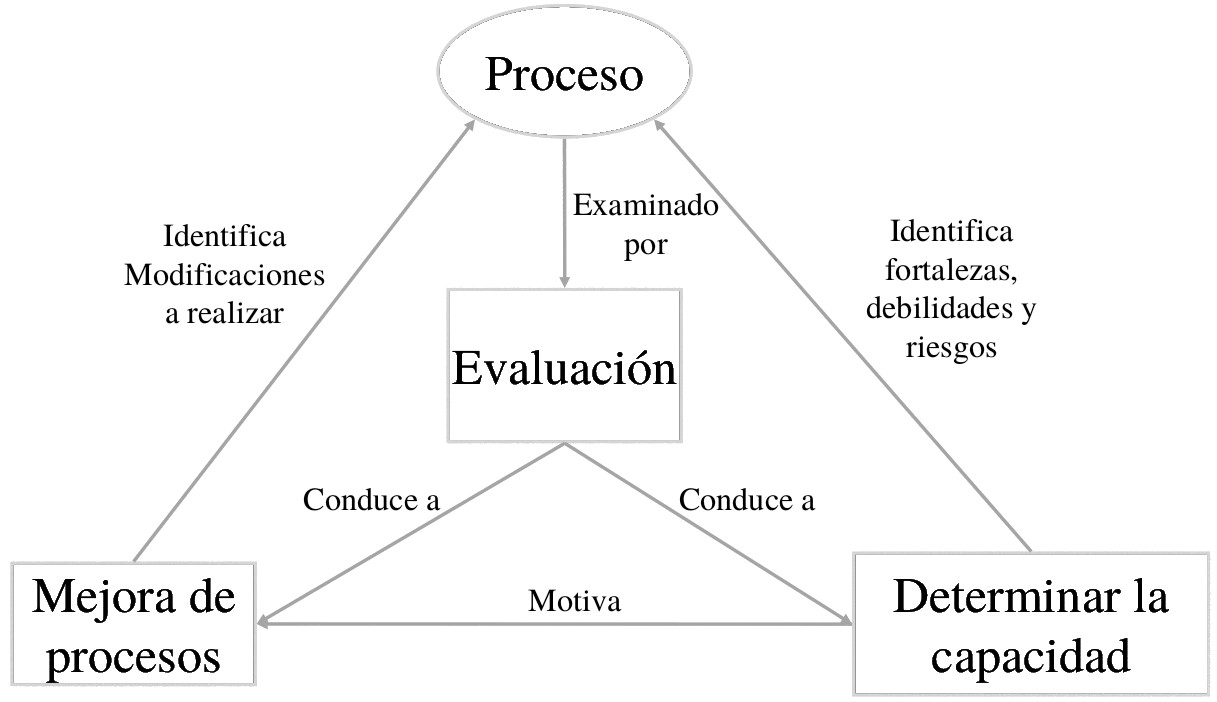
\includegraphics[width=0.7\linewidth]{Resources/evaluacionSoftware}
    \caption{Esquema de la evaluación del proceso software.}
    \label{fig:evaluacionSoftware}
\end{figure}

\subsection{Capability Maturity Model Integration (CMMI)}

Es un modelo que centra su evaluación en un total de 22 \textbf{áreas del proceso} categorizadas en:

\begin{itemize}
    \item Gestión de procesos.
    \item Gestión de proyectos.
    \item Ingeniería.
    \item Soporte.
\end{itemize}

Existen dos versiones del modelo:

\paragraph{Modelo continuo} Define el nivel de \uline{capacidad de cada una de las áreas del proceso} (es decir, de manera independiente). Los niveles de capacidad son los siguientes:
\begin{enumerate}
    \setcounter{enumi}{-1}
    \item \textbf{Incompleto}: El área del proceso aún no se realiza, o todavía no alcanza todas las metas.
    \item \textbf{Realizado}: Todas las metas del área (específicas) han sido satisfechas.
    \item \textbf{Gestionado}: Además, el trabajo del área se ajusta a una política organizacional definida (control, revisión y evaluación), y se implica al cliente cuando sea necesario.
    \item \textbf{Definido}: Además, el proceso contribuye al proceso organizacional.
    \item \textbf{Cuantitativamente gestionado}: Además, el área se controla y mejora mediante mediciones cuantitativas.
    \item \textbf{En optimización}: Ademas, el área se adapta y mejora mediante medios cuantitativas a las necesidades cambiantes del cliente.
\end{enumerate}

Cada área del proceso consta de un conjunto de \textbf{metas específicas} a alcanzar en ella, así como las \textbf{prácticas específicas} requeridas para alcanzar dichas metas (las prácticas convierten una meta en un conjunto de actividades); mediante estas metas, se pretende establecer las características que deben existir para que las actividades del área del proceso sean efectivas. Además de las metas y prácticas específicas, CMMI define \textbf{metas genéricas} y \textbf{prácticas genéricas} que se aplican a todas las áreas.\\

Esta versión del modelo cuenta con cinco metas y prácticas genéricas, cada una correspondiente a un nivel de capacidad; por ello, para alcanzar una nivel de capacidad particular, se debe alcanzar la meta genérica para dicho nivel:

\begin{enumerate}
    \item Alcanzar las metas específicas.
    \item Institucionalizar un proceso de gestión.
    \item Institucionalizar un proceso definido.
    \item Institucionalizar un proceso manejado en forma cuantitativa.
    \item Institucionalizar un proceso de mejora.
\end{enumerate}

\paragraph{Modelo discreto} Define el nivel de \uline{madurez global de los proyectos y de la organización}. Aquí, surge la principal diferencia entre las dos versiones, dado que el modelo discreto establece cinco niveles de madurez, en vez de cinco niveles de capacidad:

\begin{enumerate}
    \item Nivel por defecto.
    \item Se deben cumplir las metas generales 2 para cada para siete áreas del proceso.
    \item Se deben cumplir las metas generales 2 y 3 para 18 áreas del proceso.
    \item Solo añade 2 áreas del proceso, que deben cumplir las metas generales 2 y 3.
    \item Solo añade 2 áreas del proceso, que deben cumplir las metas generales 2 y 3.
\end{enumerate}

A diferencia del modelo continuo, del modelo discreto solo define las metas generales 2 y 3, yal y como se habían descrito.

\paragraph{Standard CMMI Appraisal Method for Process Improvement (SCAMPI)}

Método oficial mediante el cual realizar análisis de calidad en CMMI, con el objetivo de identificar los puntos fuertes y débiles de procesos, revelar riesgos, y determinar los niveles de capacidad y madurez.\\

\textbf{Nota:} \textit{la diferencia entre las dos versiones es meramente organizacional, y los contenidos equivalentes. En el modelo continuo, CMMI recomienda un orden para la mejora de los procesos a nivel de cada área, dando la libertad de escoger el orden que mejor se ajuste a la organización. En el modelo discreto, cada área tiene un único objetivo específico, y el alcanzarlo supone haber mejorado todas las actividades asociadas a él.}